With the design in chapter \ref{chap_design},
it is not hard to develop an implementation of
the swarm control and task coordination algorithm.
Specific details of different implementations may vary,
but as long as they conform to the design,
they should be able to solve the problem raised in chapter \ref{chap_problem},
and demonstrate the feasibility of the design of a dynamic hierarchical swarm.

In this thesis, the design is implemented in the Rust programming language \parencite{Rust}.
Rust is a relatively young programming language.
The first stable version of Rust was released in 2015, less than 10 years ago.
However, it soon became popular due to its safety, performance,
modern syntax, and powerful compiler.
In 2022, Rust became the third language for Linux kernel development.
Rust excels in system programming and embedded programming,
so it is very suitable for writing code which runs on a UAV controller.

The GitHub link of the project is \url{https://github.com/NGC0001/AutoSwarm}.
The project has more than 2000 lines of source code.
Appendix \ref{app_code} gives an overview of the code.
Some of the interesting implementation details are introduced in this chapter.

\section{Messages}

Messages are sent by a UAV to other UAVs, or by the GCS to a UAV.
A message is an object of struct type $Msg$.
$Msg$ has 3 fields as below.
\begin{itemize}
    \item An object of struct type $NodeDesc$
          which contains the basic information of the sender.
          $NodeDesc$ further has the following member fields.
          \begin{itemize}
              \item NID of the sender.
              \item Position of the sender.
              \item Velocity of the sender.
              \item The size of the swarm it is in.
              \item Its current task ID.
                    The type of this field is $Option$<$u32$>,
                    with $None$ meaning free and $Some(tid)$ meaning some task of ID $tid$.
          \end{itemize}
    \item A list of UAV IDs designating the receivers of the message.
    \item The message body of enum type $MsgBody$.
\end{itemize}

Different variants of $MsgBody$ represent different purposes of the message,
and contain different information.
Some important variants are as follows.
\begin{itemize}
    \item $Empty$. The message contains no extra data.
          This variant is used for broadcasting basic status of the sender.
          The information contained in the $NodeDesc$ is sufficient.
          The receiver list is empty.
    \item $Connection$. This is a connection message.
          It is used for periodic exchange of information between a child-parent pair.
          The information sent by a child to its parent
          includes sub-swarm size and sub-swarm task state.
    \item $Join$. The sender requests to set the receiver as its parent node.
    \item $Accept$. Response to $Join$. The sender accepts the receiver's request.
    \item $Reject$. Response to $Join$. The sender rejects the receiver's request.
    \item $Leave$. The sender informs the receiver, which is the current parent of the sender,
          that it is leaving the current swarm.
    \item $Task$. This message contains a task sent by the GCS.
    \item $Subtask$. The sender allocates a sub-task to the receiver,
          which is a child of the sender.
\end{itemize}

% Unreliable network communication:
%   Messages are sent based on state, rather than based on events.
%   Effect of an event-based message shall be revocable in case the message gets lost.

\section{Limit on Child-Adding Rate}

Initially at time $t = 0$, all UAVs are single-node trees.
After they are aware of the existence of each other,
they start to execute the swarm-switching algorithm.
According to algorithm \ref{alg:swarm-switching},
since all existing trees are of size 1,
the UAV with the smallest ID becomes the switching target of all other UAVs.
Hence, it is quite likely that the resulting swarm tree is a very flat one,
where the UAV with the smallest ID is the root, and it has many child nodes.
If a node has too many children,
the communication and computation overhead of the parent node will be high.

A simple solution to this problem is to set limit on the rate of adding child.
Consider three UAVs $U_i$, $U_j$, and $U_k$.
$U_i$ is closer to $U_j$ than to $U_k$.
$U_i$ and $U_j$ both send $Join$ messages to $U_k$.
$U_k$ accepts $U_j$, but rejects $U_i$ due to the limit on child-adding rate.
Then the next time $U_i$ tries to join the tree of $U_k$,
it finds that $U_j$ is also on the tree.
Since $U_j$ is closer, according to algorithm \ref{alg:swarm-switching},
$U_j$ is a better choice than $U_k$,
so it sends a $Join$ message to $U_j$, instead of to $U_k$.
In this way, the probability is greatly reduced for $U_k$ to accumulate too many children.

At time point $t$,
suppose UAV $U_i$ added child at time point $\{t_l|l = 1, \ldots, L; 0 < t_l < t\}$.
The child-adding rate for $U_i$ is
\begin{equation}
    A_i(t) = \sum_{l = 1}^{L} e^{\frac{t_l - t}{t_s}},
\end{equation}
where $t_s$ is a configurable time scale factor.
If $A_i(t)$ is greater than the preset limit $A_L$,
$U_i$ rejects any $Join$ message at time $t$.

In the software, $A_i(t)$ is easier to calculate than it seems to be.
During the time period from $t1$ to $t2$, if no child is added,
$A_i(t)$ has the following property
\begin{equation}
    A_i(t') = A_i(t1) e^{\frac{t1 - t'}{t_s}}, t1 < t' < t2.
\end{equation}
With this property, the calculation and utilisation of child-adding rate
is shown in algorithm \ref{alg:child-adding-rate}.

\begin{algorithm}
\caption{Limit on child-adding rate.}
\label{alg:child-adding-rate}
\begin{algorithmic}[1]
\State $interval \gets$ time interval of software main loop
\State $tscale \gets$ time scale factor
\State $limit \gets$ preset child-adding rate limit
\State $rate \gets 0$
\State $t \gets$ current system time
\While{true} \Comment{The main loop of the onboard software}
    \State $t\_prev \gets t$
    \State $t \gets$ current system time
    \State $rate \gets rate \times \exp((t\_prev - t) / tscale)$
    \For{$msg$ in received $Join$ messages}
        \If{$rate < limit$}
            \State accept($msg$)
            \State $rate \gets rate + 1$
        \Else
            \State reject($msg$)
        \EndIf
    \EndFor
    \State sleep\_for($interval$)
\EndWhile
\end{algorithmic}
\end{algorithm}

\section{Task Division}
\label{sec:tsk_div}

For general swarm tasks,
a good task allocation algorithm ensures that
work load is reasonably balanced across the swarm.
Besides, the algorithm shall also be fast and efficient,
to save computing power and increase swarm reaction speed.
However, task allocation algorithms usually require
sophisticated optimisation methods \parencite{Li2023, Peng2021}.

For a task defined in this thesis,
a shape is divided, and different parts are allocated to different UAVs.
A good shape division algorithm ensures that UAVs are distributed evenly on a shape,
that the flight path for each UAV is optimal,
and that each child is within the communication range of its parent.
However, the main goal of the implementation is to demonstrate that
hierarchical task coordination is viable,
not to optimise the process of coordination.
Therefore, this implementation only focuses on the even distribution problem,
with all other problems ignored.

The shape division works in two steps.
First, calculate how many UAVs are needed by each line of the shape.
Next, decide which child sub-swarm goes to which lines according to the calculation result.

The first step works in a way similar to algorithm \ref{alg:uav-dist}.
In the algorithm, the line\_length\_of function calculates the length of a line,
which is the sum of the lengths of individual line segments.
The returned $dist\_uavs$ is an array containing the number of UAVs needed by each line.
This heuristic algorithm does not ensure that
the UAVs are distributed in the most even way,
but it is simple and straightforward.

\begin{algorithm}
\caption{Calculation of UAV distribution among the lines.}
\label{alg:uav-dist}
\begin{algorithmic}[1]
\Require number of UAVs no less than number of lines
\Function{CalculateUavDistribution}{}
\State $arr\_lines \gets$ the array of lines of the shape
\State $num\_uavs \gets$ number of UAVs in the sub-swarm
\State $num\_lines \gets$ number of lines in $arr\_lines$
\State $dist\_uavs \gets$ an empty array
\For{$u$ in range $[0, num\_lines)$}
    \State $dist\_uavs.\text{push\_back}(1)$ \Comment{Each line needs at least 1 UAV}
\EndFor
\For{$u$ in range $[num\_lines, num\_uavs)$}
    \State $i \gets \displaystyle \argmax_{j \in [0, num\_lines)}
        \text{line\_length\_of}(arr\_lines[j]) / dist\_uavs[j]$
    \State $dist\_uavs[i] \gets dist\_uavs[i] + 1$
\EndFor
\EndFunction
\State \Return $dist\_uavs$
\end{algorithmic}
\end{algorithm}

The second step is to allocate the top node and its child sub-swarms onto the lines
according to the numbers of UAVs needed by the lines.
No optimisation is performed for this step.
The lines and the child sub-swarms are trivially matched one by one.
A line may be split where needed.
Figure \ref{fig:shape_div} illustrates how this step works.

\begin{figure}[htbp]
  \centering
  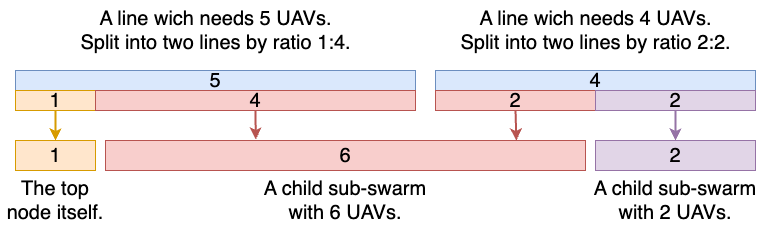
\includegraphics[width=0.9\linewidth]{rsc/shape_division.png}
  \caption[Shape division.]
  {A shape with two lines is divided into 3 parts,
  one for the top node itself,
  the other two for the two child sub-swarms.}
  \label{fig:shape_div}
\end{figure}

After the shape division process has been performed layer by layer down the tree,
each node gets its own line.
It can choose a suitable point on the line as its target point,
e.g., the middle point of the line.

% \section{Velocity Control}

% task velocity
% connection velocity
% velocity coordination
% Collision avoidance

\section{Testing}

Testing is an important part of software development.
However due to a tight schedule,
this implementation has not been systematically tested.
The overall correctness is ensured by the following two aspects.
\begin{enumerate}
    \item Black box testing. Simulations are carried out in chapter \ref{chap_sim}.
          The results turn out as expected.
    \item The safety features of Rust and the powerful static analysis of Rust compiler.
          As long as unsafe blocks are not used, Rust ensures that the code is memory safe.
          Whereas in programming languages such as C and C++,
          memory safety is the main source of bugs.
\end{enumerate}
Nevertheless, small bugs may still exist in the code.
So systematic testing, especially unit testing, should be carried out in the future.